% Kelompok Sejarah Benua dan Koordinat
% Agien Farhan S (1154012)
% Berlin Mitra Putra A (1154061)
% Indra Riksa Herlambang (1154051)
% Indra Saryoni Simanjuntak (1154115)
% Kindi Herdiansyah (1154048)

\section{Sejarah Benua}

\subsection{Benua pertama}
Mantel konveksi, proses yang mendorong lempeng tektonik adalah hasil dari aliran panas dari dalam bumi ke permukaan bumi \cite{suryasejarah}.Termasuk juga penciptaan lempeng tektonik di pegunungan bawah laut. Lempeng ini dihancurkan oleh subduksi di zona subduksi. Pada awal eon Arkean \ref{PetaAmerikaUtara} (sekitar 3 miliar tahun yang lalu) mantel itu jauh lebih panas mungkin sekitar 1600° C, sehingga proses konveksi terjadi lebih cepat.

Kerak bumi mulai terbentuk saat permukaan bumi mulai memadat, menghilangkan bekas-bekas pergeseran lempeng tektonik Hadean. Namun, diperkirakan kerak bumi memiliki komposisi Basalt seperti Kerak samudera .Potongan kerak benua besar yang pertama, muncul saat akhir masa Hadean, sekitar 4 miliar tahun yang lalu.  Kraton adalah bagian kecil yang tersisa dari benua pertama. Potongan-potongan yang terjadi pada akhir Hadean sampai awal Arkean membentuk inti lempengan yang tumbuh menjadi benua seperti sekarang.

Batuan tertua ditemukan di Laurentia, Kanada, yang berupa tonalit yang berumur sekitar 4 miliar tahun. Bebatuan ini menunjukkan jejak metamorfosis oleh suhu tinggi,  dan biji-bijian sedimen yang terkena erosi selama terbawa oleh air, yang menunjukkan terdapat sungai dan laut pada 4 miliar tahun yang lalu.

\begin{figure}[ht]
    \centerline{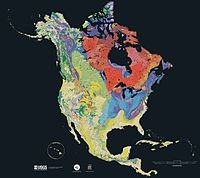
\includegraphics[width=1\textwidth]{figures/PetaAmerikaUtara.JPG}}
    \caption{Peta geologi Amerika Utara, kode warna menunjukan usia. Warna merah dan pink menunjukkan batuan dari masa eon Arkean.}
    \label{PetaAmerikaUtara}
    \end{figure}


\subsection{Benua raksasa pada masa Proterozoikum} 
Rekonstruksi pergerakan lempeng tektonik pada 250 juta tahun terakhir ( pada era Kenozoikum dan mesozoikum) dapat dilakukan dengan melihat kecocokan benua, anomali magnetik dasar laut, dan kutub paleomagnetik \cite{suryasejarah}. Para ahli tidak menemukan kerak samudera yang terbentuk sebelum waktu tersebut, sehingga rekonstruksi sebelum waktu tersebut sulit untuk dilakukan. Kutub paleomagnetik dilengkapi dengan bukti geologi seperti sabuk orogenik, yang menandai tepi lempeng kuno, dan distribusi flora dan fauna pada masa itu.

Sepanjang sejarah bumi, ada saat dimana benua bertabrakan dan membentuk benua raksasa, yang kemudian pecah menjadi benua baru. Sekitar 1000–830 juta tahun yang lalu, benua yang paling luas bersatu membentuk sebuah benua raksasa Rodinia. Sebelum Rodinia terbentuk, diperkirakan telah terbentuk terlebih dahulu Columbia atau Nuna pada awal sampai pertengahan masa Proterozoikum.

Setelah Rodinia pecah sekitar 800 juta tahun lalu, benua-benua tersebut kemungkinan telah membentuk benua raksasa lain yang berumur pendek yaitu , Pannotia \ref{BenuaRaksasaPannotia} pada 550 juta tahun lalu. Hipotetis benua raksasa mengacu pada Pannotia atau Vendia. Bukti yang memperkuat hipotesis tersebut adalah fase tabrakan benua yang diketahui sebagai orogeni Pan-Afrika, yang bergabung dengan benua Afrika , Amerika Selatan, Antartika dan Australia. Keberadaan Pannotia ditentukan oleh terjadinya retakan antara Gondwana (sebagian besar termasuk daratan di belahan bumi selatan, serta meliputi Semenanjung Arab dan anak benua India) dan Laurentia (kira-kira setara dengan Amerika Utara pada masa sekarang).Hal ini meyakinkan bahwa pada akhir masa eon Proterozoikum, sebagian besar benua bergabung dalam posisi di sekitar kutub selatan.

\begin{figure}[ht]
    \centerline{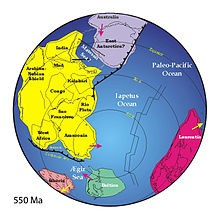
\includegraphics[width=1\textwidth]{figures/BenuaRaksasaPannotia.JPG}}
    \caption{Rekonstruksi benua raksasa Pannotia (warna kuning) pada 550 juta tahun lalu.}
    \label{BenuaRaksasaPannotia}
    \end{figure}


\subsection{Bukti Tersusunnya Benua Kuno}
Terdapat bukti dari para ahli yang digunakan untuk memperkirakan tersusunnya benua kuno.
Menurut Alfred Wegener(1880-1930), bahwa semua benua pernah bersatu kemudian berpecah menjadi sekarang ini dan benua yang bersatu itu dinamakan Pagaea (Benua Besar)\cite{hallam1975alfred}. Kemudian para ahli meneliti tentang benua dan membuat spekulasi-spekulasi teoritis yaitu melihat pada peta bahwa benua saling melengkapi dilihat dari garis pantai yang saling melengkapi seperti bagian puzzle. Kemudian meneliti fosil, bukti lain dari kehidupan lampau yaitu Mesosaurus. Mesosaurus adalah reptilia purba yang hanya hidup di air tawar dan ternyata hanya ada dua kawasan didunia yang memiliki fosil Mesosaurus ini yaitu Pantai Timur Amerika Selatan dan Pantai Barat Afrika. Kesimpulannya, fosil yang sama telah ditemukan di dalam batuan di kedua sisi lautan. Kemudian bukti korelasi batuan dan pegunungan telah ditemui di kedua belah sisi lautan. Yaitu meneliti banjaran pegunungan di Timur Laut Amerika Serikat dan banjaran pegunungan di Utara Eropa. Keduanya sangat sepadan atau keduanya tersusun daripada jenis batuan yang sama. Kemudian bukti data iklim masa lalu, terbukti pada Glacial Striations atau terdapat bentuk goresan pada batuan dan ini dapat dilihat dari hutan hujan tropika Amerika Selatan dan Afrika saat ini terdapat goresan glasier. Kesimpulannya adalah arang batu telah ditemukan di kawasan sejuk dan bukti glasier telah ditemui di kawasan panas berarti sebelumnya ada kemungkinan benua bersatu.

\section{Sejarah Koordinat}
Menurut ahli sejarah yang bernama Heroditus (450 M) menyatakan bahwa geometri berasal dari Mesir. Rane Discartes seorang matematikawan, yang lahir di sebuah Desa La Haye Prancis pada tahun 1596, adalah orang yang memiliki ketertarikan di bidang geometri. Rane Descrates telah menemukan sebuah metode untuk menyajikan sebuah titik sebagai bilangan berpasangan pada sebuah bidang datar. Bilangan-bilangan tersebut terletak pada dua garis yang saling tegak lurus antara satu dengan lainnya dan berpotongan di sebuah titik (0,0) dinamakan Origin , dan biasanya disimbolkan dengan huruf kapital O (0,0).
Bidang tersebut dinamakan bidang KOORDINAT atau yang lebih dikenal dengan bidang KARTESIUS.

\section{Sistem Koordinat}
Sistem koordinat dimaksudkan untuk memberikan peng-alamat-an terhadap setiap lokasi di permukaan bumi. Peng-alamatan dengan sistem kordinat didasarkan atas jarak timur-barat dan utara-selatan suatu tempat dari suatu titik pangkal tertentu. Jarak diukur dalam satuan derajat sudut yang dibentuk dari dari titik pangkal ke posisi tersebut melalui pusat bumi. Sedangkan titik pangkal ditetapkan berada di
perpotongan belahan utara-selatan bumi (garis katulistiwa) dengan garis yang membelah bumi timur- barat\cite{zuhdi2012sistem}.

Koordinat diambil untuk menjadi bilangan riil dalam matematika dasar, tetapi mungkin bilangan kompleks atau elemen-elemen dari sistem yang lebih abstrak. Penggunaan sistem koordinat memungkinkan masalah dalam angka untuk diterjemahkan ke dalam masalah-masalah tentang geometri dan juga sebaliknya.

\subsection{Sistem Koordinat Dua Dimensi}
\subsubsection{Sistem Koordinat Kartesius}
Koordinat Cartesius bukan merupakan satu-satunya jalan untuk menunjukkan kedudukan suatu titik pada bidang. Karena bentuk geometris di alam tidak selalu berupa kotak-kotak atau persegi panjang, namun adakalanya berbentuk lingkaran\cite{mufidah2015solusi}.Sistem koordinat Kartesius pada dua dimensi umumnya didefinisikan dengan dua buah sumbu yang saling tegak lurus antara satu dengan yang lainnya, yang keduanya terletak pada satu bidang (bidang xy). Sumbu horizontal(x), dan sumbu vertikal(y). Lalu, pada sistem koordinat tiga dimensi, ditambahkan sumbu yang lain yang sering diberi label z. Sumbu-sumbu tersebut ortogonal antar satu dengan yang lainnya. Titik pertemuan antara kedua sumbu, titik asal, pada umumnya diberi label 0. Setiap sumbu juga memiliki besaran panjang unit, dan setiap panjang tersebut diberi tanda dan membentuk semacam grid. Untuk mendeskripsikan suatu titik tertentu pada sistem koordinat dua dimensi, nilai absis(x), lalu diikuti dengan nilai ordinat(y). Dengan demikian, format yang dipakai selalu (x dan y) dan urutannya tidak dibalik-balik.

Gambar \ref{koordinat} Tanda panah yang ada pada sumbu berarti panjang sumbunya tak terhingga pada arah panah tersebut.

\begin{figure}[ht]
    \centerline{\includegraphics[width=1\textwidth]{figures/koordinat.JPG}}
    \caption{Keempat kuadran sistem koordinat Kartesius}
    \label{koordinat}
    \end{figure}

Pilihan huruf-huruf didasari oleh konvensi, yaitu huruf-huruf yang dekat akhir(x dan y) yang digunakan untuk menandakan variabel dengan nilai yang tidak diketahui, sedangkan huruf-huruf yang lebih dekat awal digunakan untuk menandakan nilai yang diketahui. Karena kedua sumbu saling bertegak lurus satu sama lain, bidang xy terbagi menjadi empat bagian yang disebut dengan kuadran, yang pada Gambar 3 ditandai dengan angka I, II, III, dan IV. Menurut konvensi yang berlaku, keempat kuadran tersebut diurutkan mulai dari yang kanan atas (kuadran I), melingkar melawan arah jarum jam (lihat Gambar 3). Pada kuadran I, kedua koordinat (x,y) bernilai positif. Pada kuadran II, koordinat x bernilai negatif dan koordinat y bernilai positif. Pada kuadran III, kedua koordinat mempunyai nilai negatif, dan pada kuadran IV, koordinat x bernilai positif dan y bernilai negatif. (lihat gambar \ref{contoh} dibawah ini).

\begin{figure}[ht]
    \centerline{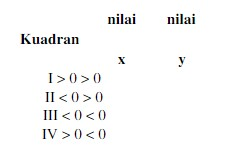
\includegraphics[width=1\textwidth]{figures/contoh.JPG}}
    \caption{Nilai x dan y pada Kuadran I,II,III,IV}
    \label{contoh}
    \end{figure}

\subsubsection{Sistem Koordinat Polar}
Pada sistem koordinat polar, sepasang koordinat polar suatu titik ditulis dengan (𝑟,𝜃)\cite{mufidah2015solusi}.Konsep dari sudut dan radius sudah diterapkan oleh orang-orang pada zaman dahulu se-abad sebelum masehi. Para astronom yunani dan astrologhipparcuhus (190-120 BCE) menemukan sebuah tabel dari fungsi dawai yang memberikan panjang dawai dari setiap sudut dan terdapat referensi dari penggunaan koordinat polar untuk mengetahui posisi bintang.

Sejak abad ke-8 yang lalu, astronom mengembangkan cara untuk mengira-ngira dan menghitung arah dari mekah, kaabah- beserta jaraknya-dari seluruh lokasi dari bumi. Penghitungan penting yaitu penggantian dari koordinat polar ekuatorial dari mekkah kedalam bentuk koordinat polar hampir sama pada sistem yang merupakan pusat dari lingkaran besar melewati daerah yang dilewati dan kutub bumi, serta sudut polar yaitu garis yang melewati daerah tersebut dan titik antipodal.

Dalam Method of fluxion (tertulis 16711) Sir Isaac Newton menentukan hubungan antara koordinat polar, yang kemudian ia sebut dengan “ tujuh cara untuk spiral, dan sembilan sistem koordinat. 

\section{Geometri Koordinat}
 Pembelajaran subtajuk-subtajuk Geometri Koordinat, iaitu jarak antara dua titik, pembahagian tembereng garis, luas poligon, persamaan garis lurus, garis lurus selari dan garis lurus serenjang, persamaan lokus yang melibatkan jarak antara dua titik dan menentukan hubungan antara pencapaian responden dalam topik pelajaran\cite{shong2013analisis}.
 
 \subsection{Sketsa Grafik Garis}
 Sketsa grafik garis merupakan salah satu materi yang membahas mengenai penggambaran grafik garis lurus pada bidang kartesius berdasarkan persamaan yang diberikan. Materi ini mirip dengan metode penggambaran garis yang ada atau diajarkan pada aljabar. Maka jika sudah menguasai materi aljabar, sketsa grafik garis bukan masalah untuk dipelajari. Dalam menggambar grafik garis lurus, pertama harus melakukan pencarian pada nilai x dan y pada bidang kartesius dari persamaan yang sudah ada. Setelah nilai x dan y pada bidang kartesius telah di-temukan tentu bisa menentukan titiknya dan langsung menggambar garis tersebut.
 
 \subsection{Persamaan Garis Lurus}
 Persamaan garis lurus dapat di-definisikan sebagai perbandingan selisih nilai x dan y yang sudah melangkahi 2 titik pada garis. 
 Persamaan garis lurus terdapat satu komponen Gradien yaitu kecenderungan sebuah garis, gradien biasa dilambangkan dengan huruf m.
 Dalam materi persamaan garis lurus terdapat materi pokok seperti menentukan \"gradien" garis lurus, \"kedudukan" garis lurus,
 \"persamaan" garis melalui satu titik merupakan gradien, dan \"persamaan" garis melalui dua titik.
 
 \subsection{Pesamaan Lingkaran}
 Persamaan lingkaran adalah persamaan titik koordinat yang membentuk sebuah lingkaran pada bidang kartesius. Pada konsep ini jari lingkaran yang telah terbentuk adalah jarak dari himpunan titik koordinat ke titik pusat atau sebaliknya.Pada persamaan lingkaran yang dapat dipelajari seperti lingkaran yang memiliki pusat (0,0), lingkaran yang memiliki pusat (a,b).
 
 \subsection{Program Linear}
 Program linear adalah metode matematika yang digunakan untuk menyelesaikan soal-soal yang memiliki batas persamaan linear. Secara umum program linear terbagi atas 2 bagian yaitu fungsi kendala dan fungsi objektif. Penyelesaian program linear model matematika adalah suatu metode penerjemahan permasalahan ke dalam bentuk matematika, sehingga soal tersebut bisa diselesaikan secara matematis.
 
 \subsection{Pembelajaran Geometri Koordinat}
 Geometri Koordinat merupakan materi yang memberika pengujian ketrampilan dalam geometri dan aljabar.
 Jika sudah menguasai materi geometri dan aljabar maka bisa dinyatakan geometri koordinat tidak lagi membuat sulit untuk dipelajari.